\documentclass[crop,tikz,12pt]{standalone}

\usepackage{tikz-qtree}
\usetikzlibrary{arrows.meta}
\usetikzlibrary{decorations.text}

\definecolor{bg1}{RGB}{244,231,195}
\definecolor{bg2}{RGB}{234,204,161}
\definecolor{l1}{RGB}{209,148,106}


\begin{document}

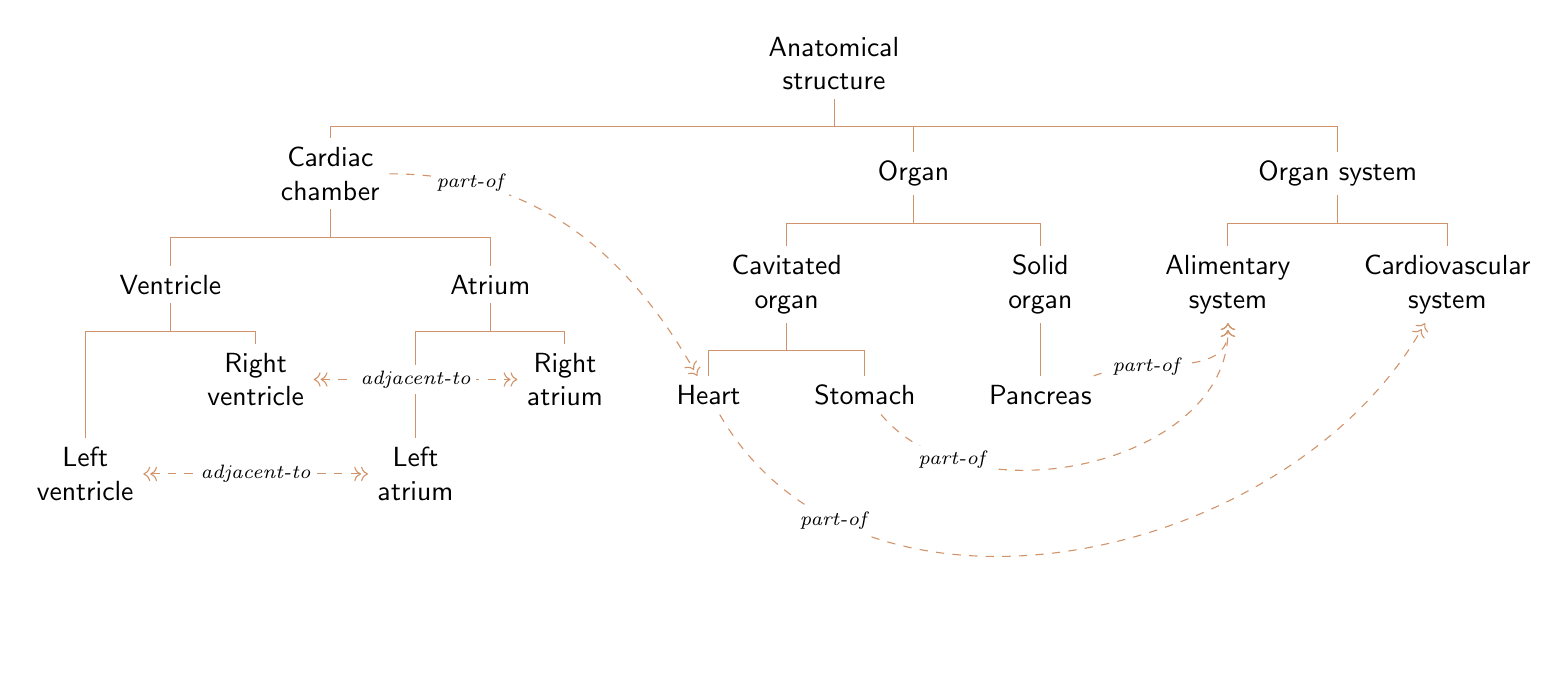
\begin{tikzpicture}[
    level distance=4em,
    sibling distance=2em,
    every tree node/.style={
        align=center, font=\sffamily
    },
    edge from parent/.append style={
        line width=0,
        color=l1
    },
    edge from parent path={
        (\tikzparentnode.south) -- +(0,-1em) -| (\tikzchildnode)
    },
    every edge/.append style={
        dashed, draw=l1,
        -{Computer Modern Rightarrow[] . Computer Modern Rightarrow[]}
    },
    b/.append style={
        {Computer Modern Rightarrow[] . Computer Modern Rightarrow[]}%
        -{Computer Modern Rightarrow[] . Computer Modern Rightarrow[]}
    },
    l/.style={
        fill=white,inner sep=0.7mm,node font=\scriptsize\itshape
    }
]
    \Tree [
        .\node (structure) {Anatomical\\structure}; [
            .\node (chamber) {Cardiac\\chamber}; [
                .\node (ventricle) {Ventricle};
                    \node (lventricle) [yshift=-1cm] {Left\\ventricle};
                    \node (rventricle) [yshift=.2cm] {Right\\ventricle};
            ] [
                .\node (atrium) {Atrium};
                    \node (latrium) [yshift=-1cm] {Left\\atrium};
                    \node (ratrium) [yshift=.2cm] {Right\\atrium};
            ]
        ] [
            .\node (organ) {Organ}; [
                .\node (cavitated) {Cavitated\\organ};
                    \node (heart) {Heart};
                    \node (stomach) {Stomach};
            ] [
                .\node (solid) {Solid\\organ};
                    \node (pancreas) {Pancreas};
            ]
        ]
        [
            .\node (system) {Organ system};
                \node (alimentary) {Alimentary\\system};
                \node (cardio) {Cardiovascular\\system};
        ]
    ]
    
    \draw (chamber)
        edge [out=0,in=120] node [l,pos=0.2] {part-of}
        (heart);
    
    \draw (lventricle)
        edge [b] node [l,pos=0.5] {adjacent-to}
        (latrium);
    
    \draw (rventricle)
        edge [b] node [l,pos=0.5] {adjacent-to}
        (ratrium);
    
    \draw (stomach)
        edge [out=310,in=270] node [l,pos=0.2] {part-of}
        (alimentary);
    
    \draw (pancreas)
        edge [out=20,in=270] node [l,pos=0.3] {part-of}
        (alimentary);
    
    \draw (heart)
        edge [out=300,in=240] node [l,pos=0.2] {part-of}
        (cardio);
    
\end{tikzpicture}

\end{document}





